\begin{figure}[t]
\cite{Westbrook:2011:PRR:2341616.2341627}
\centering
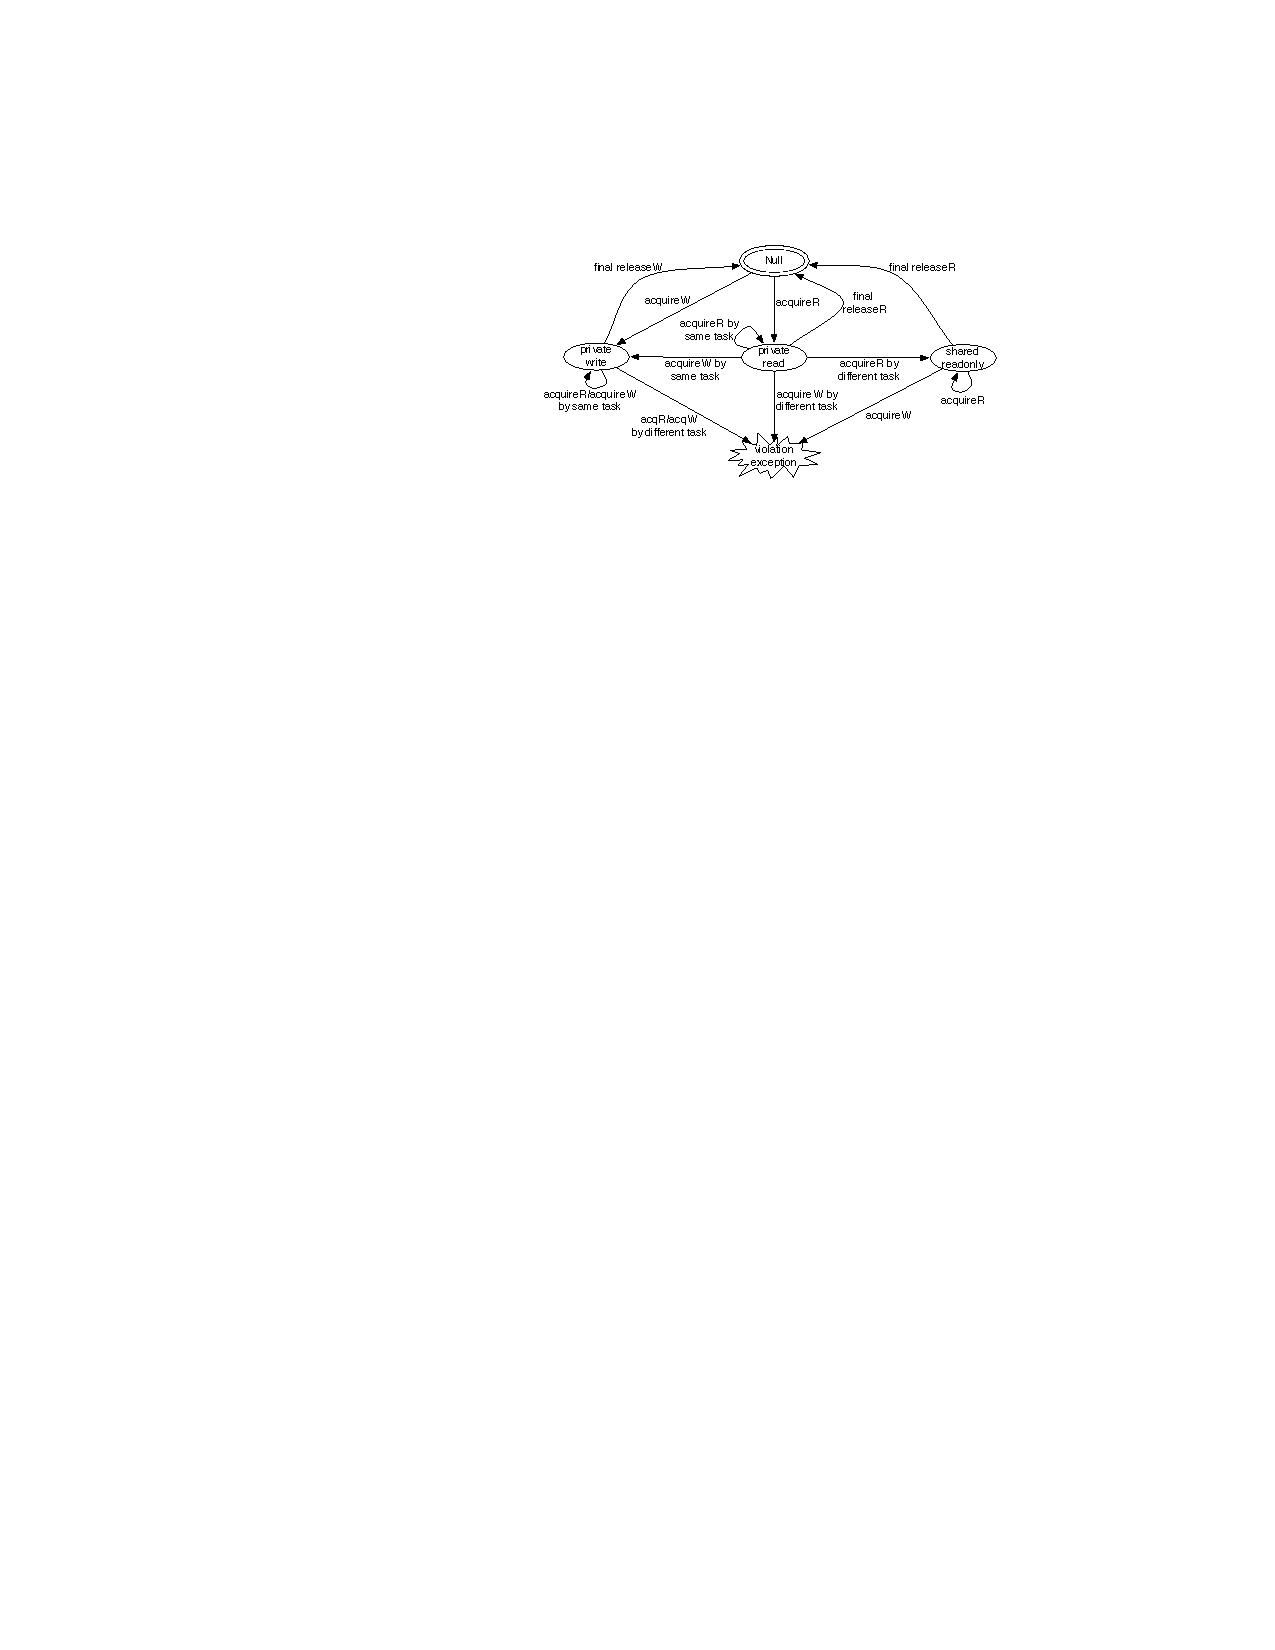
\includegraphics[width=3.25in]{../figs/state-machine}
\caption{State machine for permission regions operating on a single object}
\label{fig:state-machine}
\end{figure}

\begin{figure}[t]
\centering
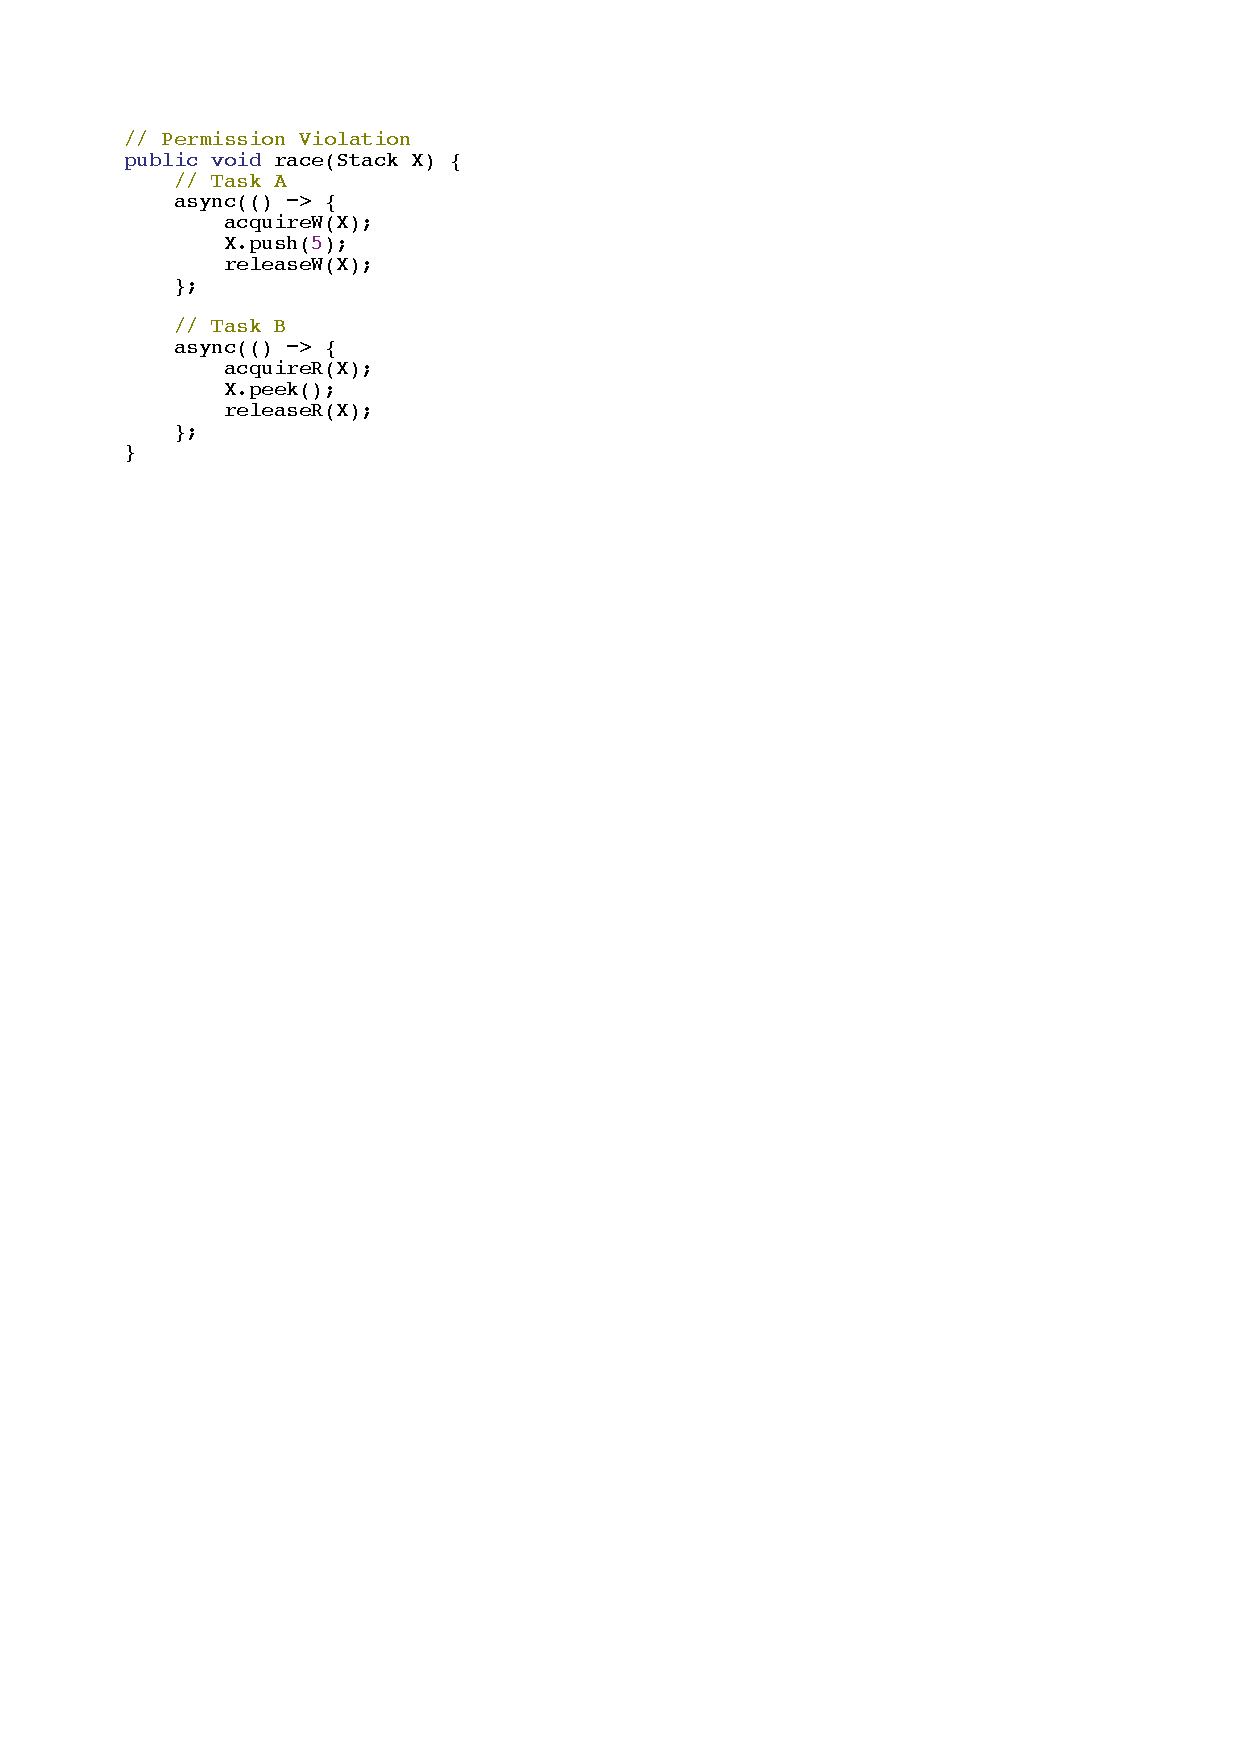
\includegraphics[width=3.25in]{../figs/permission-violation}
\caption{Permission violation while operating on a stack}
\label{fig:permission-violation}
\end{figure}

\begin{figure}[t]
\centering
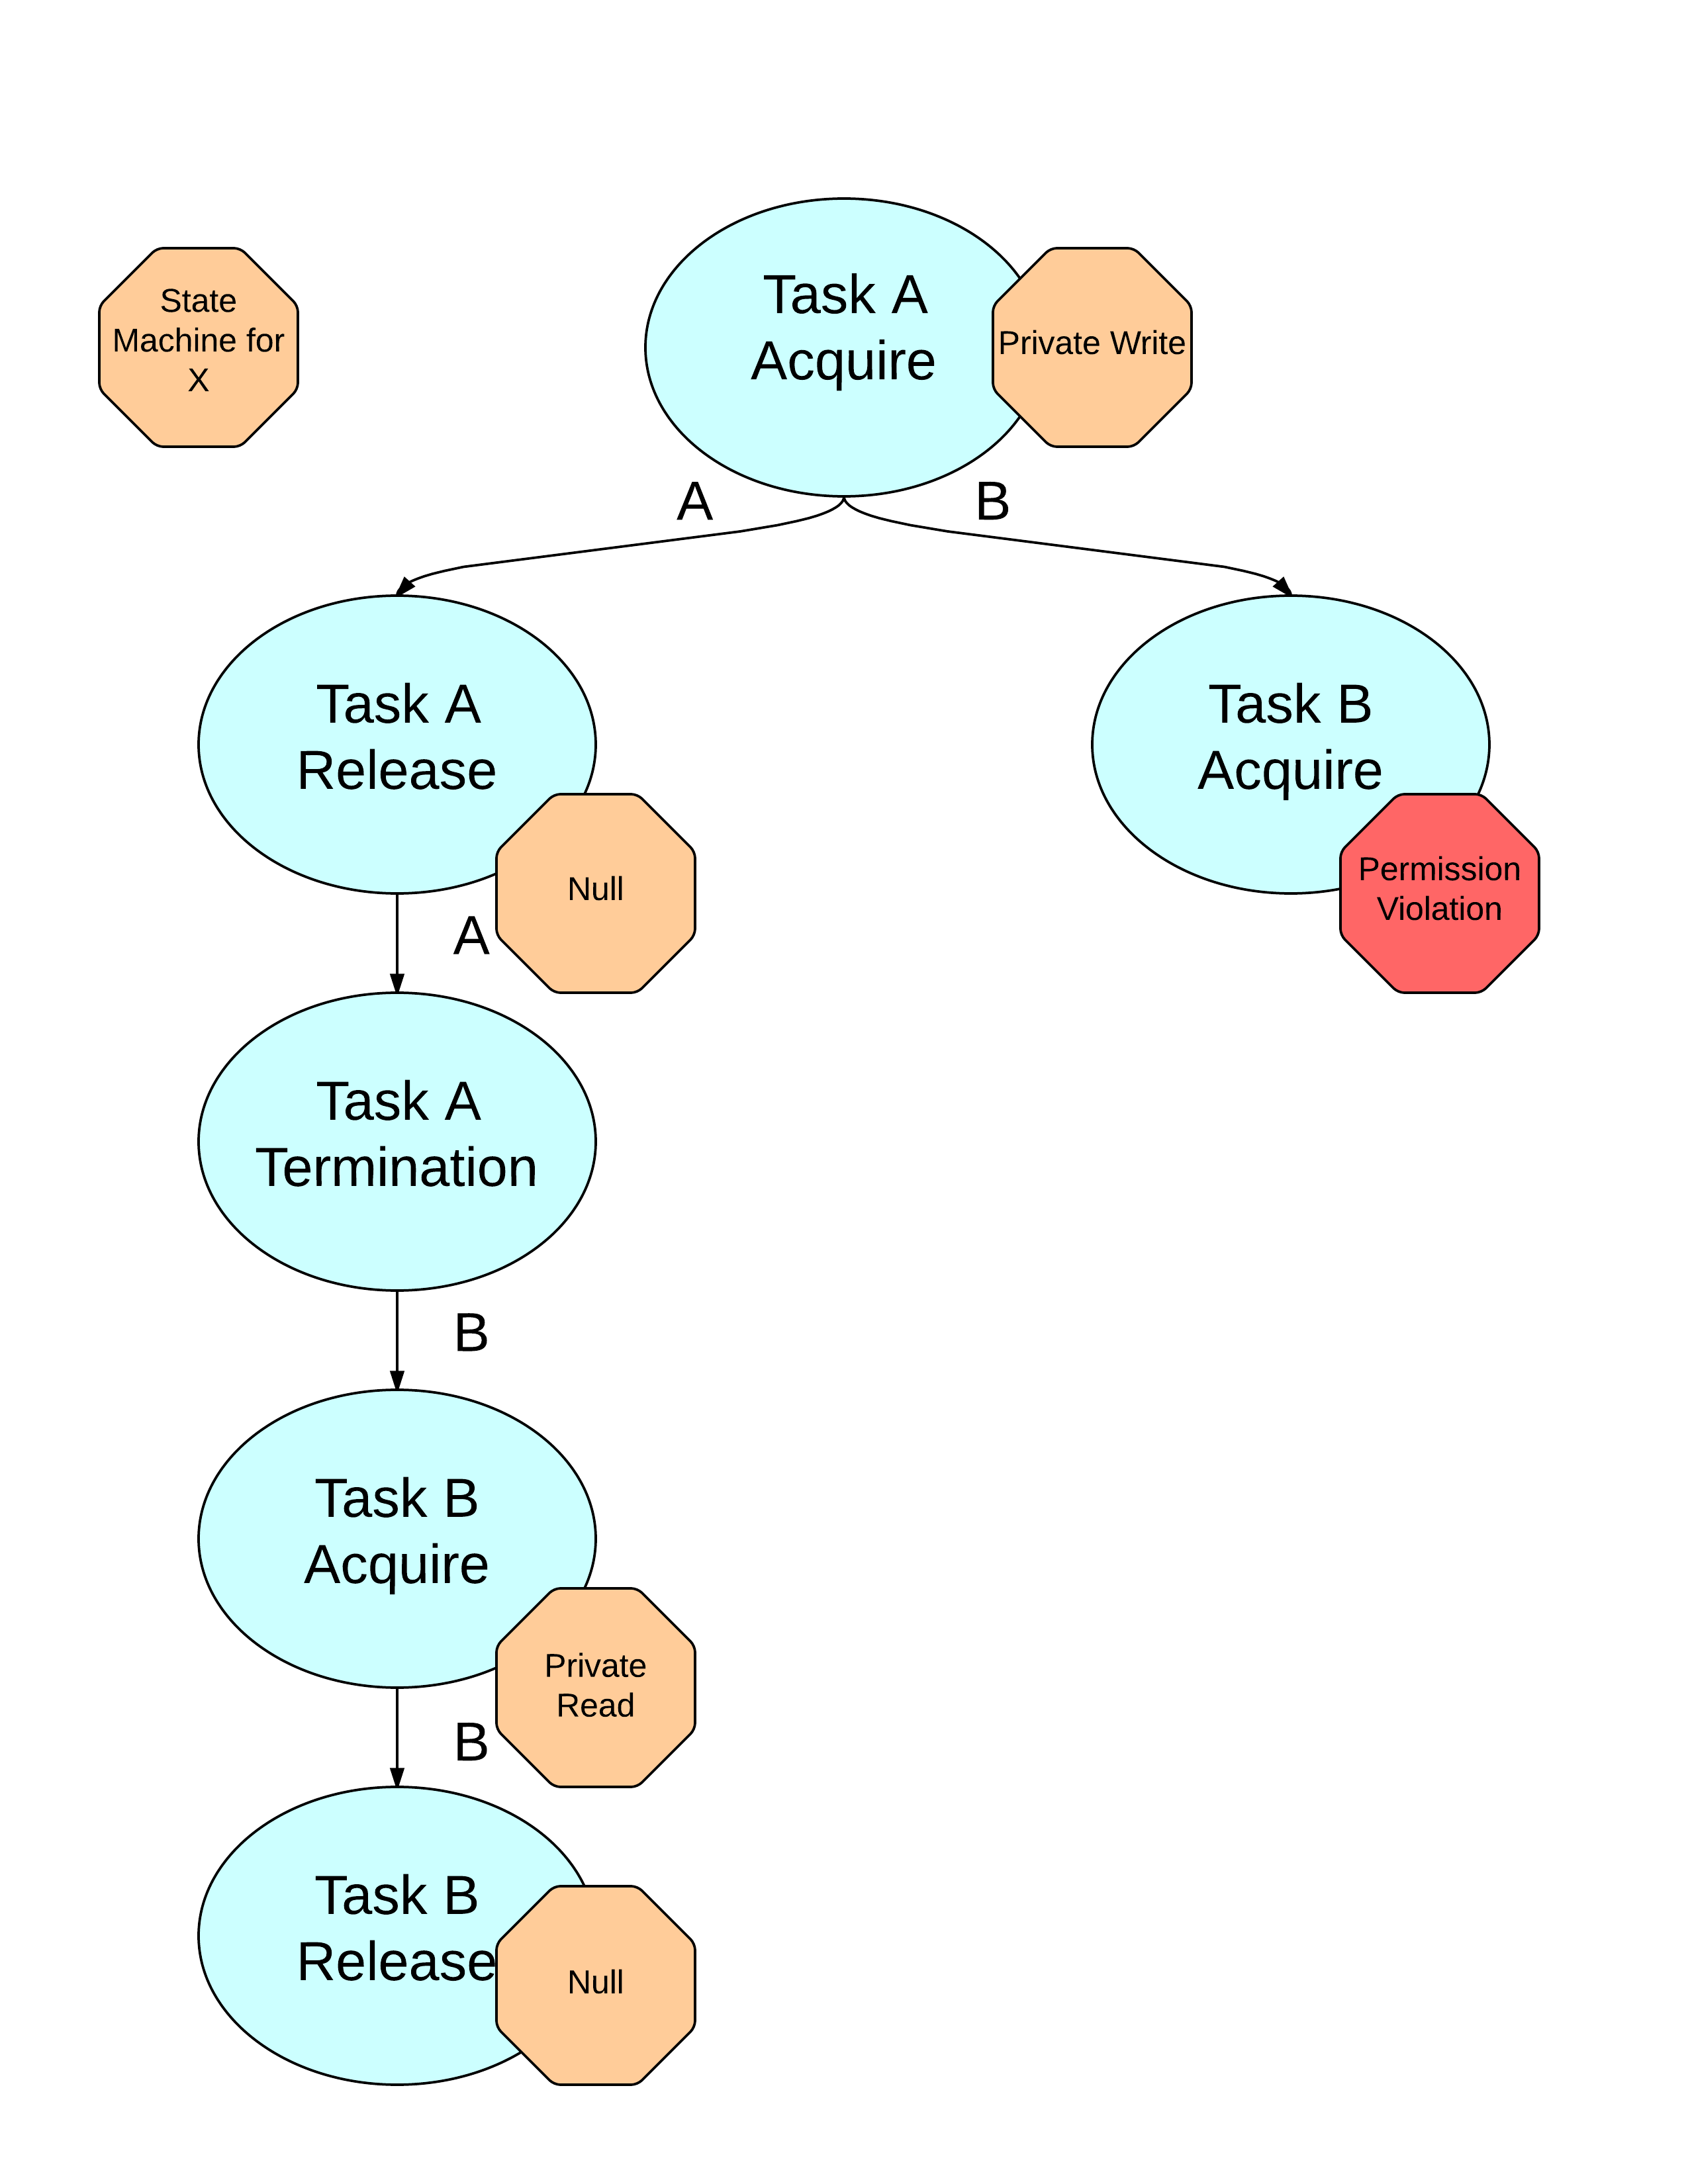
\includegraphics[width=3.25in]{../figs/permission-violation-state}
\caption{State space for permission violation example}
\label{fig:permission-violation-state}
\end{figure}


\section{JPF}

We have chosen to use a combination of a custom listener, a scheduler factory,
and attribute info to extend JPF to perform permission region verification. 
%
A brief description of each  follows.

Our listener, HjListener, extends JPF's property adapter class. Consequently it
inherits the behavior of the property adapter class, but with two modifications: 1)
executeInstruction and 2) instructionExecuted.
%
In JPF, these two methods are used to observe/modify the system state before an
instruction has been executed (executeInstruction) or after the instruction has
been executed (instructionExecuted). 
%
In both cases, the method observes whether the instruction is a permission
region relevant instruction (acquire/release).
%
In the former case, HjListener will insert a choice generator with all runnable threads enabled and in the latter case it will perform appropriate permission checks on all read/write accesses performed in the permission region on the annotated variable.
%

HjScheduler mimics the behavior of JPF's default schedule with one exception:
choice generators are not inserted when threads access shared variables.
Currently, JPF inserts shared access choice generators dynamically as it
discovers sharing. JPF relies upon the placement of these choice generators to
correctly detect race conditions. When a shared variable is discovered, JPF will
insert a choice generator at the shared variable's location. This choice
generator will cause JPF to interleave the execution of all runnable threads. If
JPF (more precisely, JPF's PreciseRaceDetector) detects simultaneous read/write
access of the shared variable it will notify the user of a data race. However,
if one of the conflicting threads is no longer runnable (terminated, blocked,
etc) then JPF will not report the error. In other words, JPF's partial-order reduction is
incomplete. In contrast, when using GPRs, programmer annotations dictate the location of the inserted
choice generators. As shown in previous work
\cite{Westbrook:2012:PPR:2367163.2367201}, a gradual type system can be used to
reduce the annotation burden for programmers.
%

HjAttribute is a series of classes that handle the actual permission
violation checks. Each object that is guarded by a permission region is assigned
an attribute info. This attribute info is an object-specific state machine. This
machine defines four valid states: Null, Private-Read, Private-Write, and
Shared-Read. See \figref{fig:state-machine}. Null is the state of an object for which no task has acquired
permissions. An object which has been acquired by a single task for read/write
permissions has state Private-Read/Private-Write respectively. Shared-Read is
the state of an object when multiple tasks concurrently acquire read
permissions.

When HjListener detects that an acquire/release statement has been executed on
object X, it signals a state transition on the state machine belonging to X. If a
legal transition is not defined then a runtime exception is thrown. 

Upon backtracking, JPF performs a shallow copy on attribute infos. This means
that the object itself will be restored, but none of the underlying changes to
the object. HjAttribute was designed to be entirely immutable (transitions from
state X to Y are simulated by replacing the machine in state X with a new
machine in state Y); therefore, when JPF backtracks, all of the
attribute infos are properly restored.

A walk-through of this system for a typical data race will highlight the
interplay among different pieces of the system.
\figref{fig:permission-violation} shows an example of concurrent accesses on a
common data structure (X). Since two threads have conflicting permission requirements
that can occur in parallel, we expect that a permission violation should be detected.

The first task to begin execution will request permission acquisition on object
X. HjListener will detect that an acquisition is pending and will insert a
choice generator at the current location in the schedule. HjListener will also
attach a state-machine to X as seen in \figref{fig:permission-violation-state}.
If task A is the first task to run then the state machine will be set to the
private write state. JPF may now choose to either execute task B or finish the
execution of task A. We will consider the case where task B is
chosen. Task B will then request permission acquisition on X.
HjListener will insert another choice generator and then will examine the state
machine attached to X. There is no transition defined from the private write
state to the private read state or vice-versa, thus an exception will be
thrown. This exception is then reported by JPF as a permission violation. Similarly, if Task B executed first, then we'd get an error when task A tried to assert write permission.
